\documentclass[12pt,a4paper]{article}

% ─── 1. PACKAGES ──────────────────────────────────────────────────────────────
\usepackage[utf8]{inputenc}
\usepackage[T1]{fontenc}
\usepackage{amsmath, amssymb}
\usepackage{geometry}
\usepackage{graphicx}
\usepackage{xcolor}
\usepackage{listings}
\usepackage{hyperref}
\usepackage{booktabs}
\usepackage{enumitem}
\usepackage{tcolorbox}
\usepackage{mdframed}
\usepackage{fancyhdr}
\usepackage{titlesec}
\usepackage{caption}
\usepackage{pgfplots}
\pgfplotsset{compat=1.18}


% Font Settings
\usepackage{newtxtext,newtxmath}
\usepackage{courier}

\geometry{margin=2.5cm}

% ─── 2. WARNA TEMA ────────────────────────────────────────────────────────────
\definecolor{codebg}{RGB}{245,247,250}
\definecolor{codeframe}{RGB}{180,195,215}
\definecolor{keywordcolor}{RGB}{0,112,192}
\definecolor{commentcolor}{RGB}{100,160,100}
\definecolor{stringcolor}{RGB}{180,70,50}
\definecolor{notebg}{RGB}{255,249,230}
\definecolor{noteframe}{RGB}{230,180,50}
\definecolor{tipbg}{RGB}{230,245,235}
\definecolor{tipframe}{RGB}{50,160,90}
\definecolor{sectioncolor}{RGB}{30,80,150}

% ─── 3. STYLE SECTION & TOC ───────────────────────────────────────────────────
\titleformat{\section}{\Large\bfseries\color{sectioncolor}}{}{0em}{\thesection\quad}[\titlerule]
\titleformat{\subsection}{\large\bfseries\color{sectioncolor!80}}{}{0em}{\thesubsection\quad}
\titleformat{\subsubsection}{\normalsize\bfseries\color{sectioncolor!60}}{}{0em}{\thesubsubsection\quad}

\usepackage{tocloft}
\renewcommand{\cftsecleader}{\cftdotfill{\cftdotsep}}
\renewcommand{\cftsecfont}{\bfseries\color{sectioncolor}}

% ─── 4. LISTINGS (CODE STYLE) ─────────────────────────────────────────────────
\lstdefinestyle{customstyle}{
  basicstyle=\ttfamily\small,
  backgroundcolor=\color{codebg},
  frame=single,
  rulecolor=\color{codeframe},
  keywordstyle=\bfseries\color{keywordcolor},
  commentstyle=\itshape\color{commentcolor},
  stringstyle=\color{stringcolor},
  numbers=left,
  numberstyle=\tiny\color{gray},
  breaklines=true,
  tabsize=4,
  showstringspaces=false
}
\lstset{style=customstyle}

% ─── 5. KOTAK CATATAN ─────────────────────────────────────────────────────────
\newmdenv[
  backgroundcolor=notebg, linecolor=noteframe, linewidth=2pt,
  leftline=true, topline=false, rightline=false, bottomline=false,
  innerleftmargin=10pt, innertopmargin=6pt, innerbottommargin=6pt, skipabove=8pt
]{notebox}

\newmdenv[
  backgroundcolor=tipbg, linecolor=tipframe, linewidth=2pt,
  leftline=true, topline=false, rightline=false, bottomline=false,
  innerleftmargin=10pt, innertopmargin=6pt, innerbottommargin=6pt, skipabove=8pt
]{tipbox}

% ─── 6. HEADER & FOOTER ───────────────────────────────────────────────────────
\pagestyle{fancy}
\fancyhf{}
\fancyhead[L]{\small\textit{Pengolahan Citra Digital -- Bab 3}}
\fancyhead[R]{\small\textit{noteify -- Pemrosesan dalam Domain Spasial}}
\fancyfoot[C]{\thepage}
\renewcommand{\headrulewidth}{0.4pt}

% ─── 7. DATA COVER ────────────────────────────────────────────────────────────
\title{
  {\LARGE\bfseries Pengolahan Citra Digital}\\[0.5em]
  {\large Bab 3: Pemrosesan Intensitas dan Penyaringan dalam Domain Spasial}\\[0.8em]
  {\normalsize Memahami teknik transformasi piksel, pemrosesan histogram, dan penyaringan spasial sebagai fondasi utama pengolahan citra.}
}
\author{}
\date{}

% ==============================================================================
\begin{document}

\maketitle
\thispagestyle{fancy}
\tableofcontents
\newpage

% ==============================================================================
\section{Pendahuluan}
% ==============================================================================

Pemrosesan dalam \textit{domain spasial} adalah salah satu pendekatan paling fundamental dalam pengolahan citra digital. Berbeda dengan domain frekuensi (seperti Fourier Transform), di sini kita bekerja langsung pada nilai piksel citra.

Secara umum, operasi pada domain spasial dapat dituliskan sebagai:
\begin{equation}
  g(x,y) = T\bigl[f(x,y)\bigr]
  \label{eq:spatial_domain_general}
\end{equation}
di mana $f(x,y)$ adalah citra masukan, $g(x,y)$ adalah citra keluaran, dan $T$ adalah operator yang bekerja pada suatu \textit{neighborhood} (lingkungan) di sekitar titik $(x,y)$.

Bab ini mencakup dua kategori besar operasi:
\begin{enumerate}
  \item \textbf{Point Processing} -- nilai piksel baru hanya bergantung pada nilai piksel itu sendiri.
  \item \textbf{Neighborhood Processing} -- nilai piksel baru bergantung pada piksel-piksel di sekitarnya (disebut \textit{spatial filtering}).
\end{enumerate}

% ==============================================================================
\section{Fondasi Matematika: Transformasi Intensitas (Bagian 3.1 \& 3.2)}
% ==============================================================================

\subsection{Intuisi Dasar}

Bayangkan setiap piksel sebagai sebuah angka tunggal yang merepresentasikan kecerahan. \textit{Transformasi intensitas} adalah sebuah fungsi yang mengambil angka lama ($r$) dan mengubahnya menjadi angka baru ($s$) berdasarkan aturan tertentu. Proses ini disebut \textbf{point processing} karena nilai baru sebuah piksel \textit{hanya} bergantung pada nilai piksel itu sendiri, bukan tetangganya.

\textbf{Rumus Umum:}
\begin{equation}
  s = T(r)
  \label{eq:intensity_transformation}
\end{equation}
di mana $r$ adalah intensitas sebelum diproses, $s$ adalah intensitas sesudah diproses, dan $T$ adalah operator transformasi.

\subsection{Jenis-Jenis Transformasi Dasar}

\subsubsection{Citra Negatif}

Membalikkan intensitas sehingga piksel terang menjadi gelap dan sebaliknya. Sangat berguna untuk menonjolkan detail putih pada latar yang gelap.

\begin{equation}
  s = (L-1) - r
  \label{eq:negative_transform}
\end{equation}


\captionsetup[figure]{labelfont=bf}

\renewcommand{\thefigure}{3.\arabic{figure}}
\setcounter{figure}{3}

\begin{figure}[h]
    \centering
    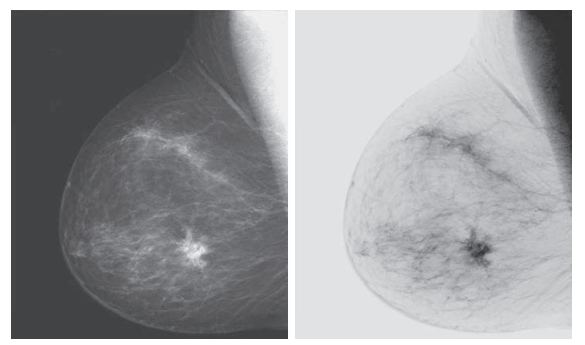
\includegraphics[width=0.5\textwidth]{3-3-4.png}
    \caption{(a) Sebuah mammogram digital. (b) Citra negatif yang diperoleh menggunakan Persamaan \ref{eq:negative_transform}.}
    \label{fig:gambar3.4}
\end{figure}


\begin{notebox}
\textbf{Contoh Aplikasi:} Citra mammogram sering diproses menggunakan negatif agar massa yang semula terlihat putih halus di latar terang menjadi lebih kontras. Lihat \textbf{[FIGURE 3.4]}.
\end{notebox}

\subsubsection{Transformasi Log}

Memperluas (memperjelas) nilai piksel gelap yang terkompresi. Sangat berguna ketika citra memiliki rentang nilai yang sangat ekstrem, seperti hasil spektrum Fourier.

\begin{equation}
  s = c \cdot \log(1 + r)
  \label{eq:log_transformation}
\end{equation}

di mana $c$ adalah konstanta skala. Karena $\log(1)=0$, nilai nol tetap dipetakan ke nol.

\begin{figure}[h]
    \centering
    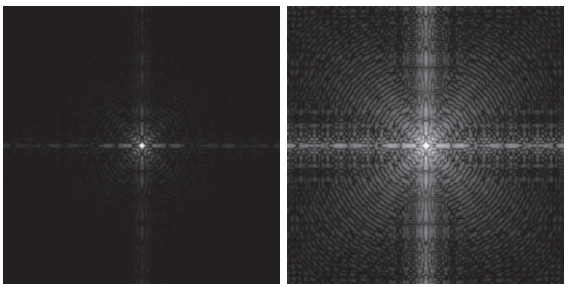
\includegraphics[width=0.5\textwidth]{3-3-5.png}
    \caption{(a) Spektrum Fourier yang ditampilkan sebagai citra skala abu-abu. (b) Hasil penerapan transformasi logaritmik pada Persamaan \ref{eq:log_transformation} dengan c=1c = 1c=1. Kedua citra diskalakan ke rentang [0, 255]..}
    \label{fig:gambar3.5}
\end{figure}


\begin{notebox}
\textbf{Contoh Aplikasi:} Menampilkan spektrum Fourier -- nilai koefisien bisa berbeda jutaan kali lipat. Tanpa transformasi log, hampir semua nilai akan tampak hitam. Lihat \textbf{[FIGURE 3.5]}.
\end{notebox}

\subsubsection{Transformasi Power-Law (Gamma Correction)}

Ini adalah \textit{``jantung''} dari kalibrasi monitor dan pengaturan kontras citra.

\begin{equation}
  s = c \cdot r^{\gamma}
  \label{eq:gamma_transformation}
\end{equation}

\begin{itemize}
  \item Jika $\gamma < 1$: area gelap \textit{diperlebar} $\Rightarrow$ citra menjadi lebih terang.
  \item Jika $\gamma > 1$: area terang \textit{diperlebar} $\Rightarrow$ citra menjadi lebih gelap dan kontras.
  \item Jika $\gamma = 1$: transformasi linier (tidak ada perubahan).
\end{itemize}

\begin{figure}[h]
\centering
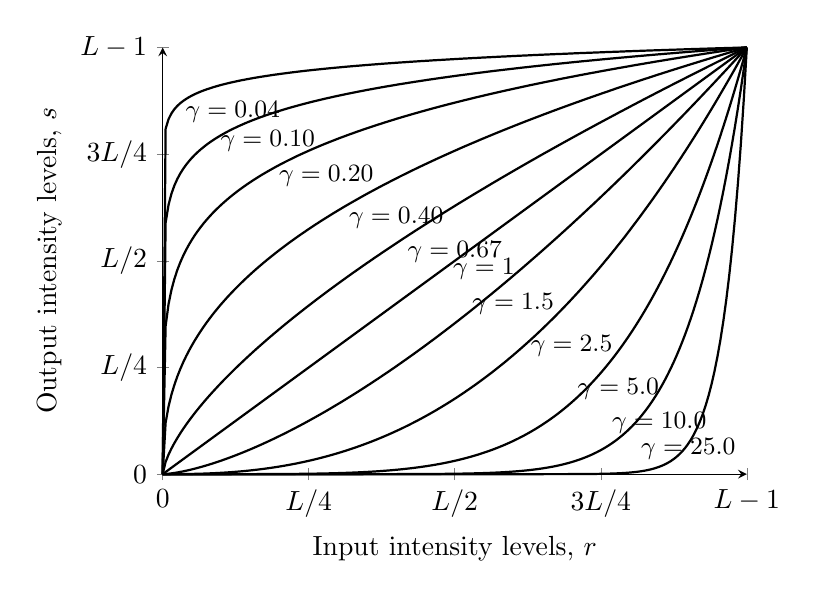
\begin{tikzpicture}
\begin{axis}[
    width=9cm,
    height=7cm,
    xmin=0, xmax=1,
    ymin=0, ymax=1,
    axis lines=left,
    xlabel={Input intensity levels, $r$},
    ylabel={Output intensity levels, $s$},
    xtick={0,0.25,0.5,0.75,1},
    xticklabels={$0$,$L/4$,$L/2$,$3L/4$,$L-1$},
    ytick={0,0.25,0.5,0.75,1},
    yticklabels={$0$,$L/4$,$L/2$,$3L/4$,$L-1$},
    samples=200,
    domain=0:1,
    clip=false
]

% kurva gamma
\addplot[thick] {x^0.04};
\node at (axis cs:0.12,0.85) {\small $\gamma=0.04$};

\addplot[thick] {x^0.1};
\node at (axis cs:0.18,0.78) {\small $\gamma=0.10$};

\addplot[thick] {x^0.2};
\node at (axis cs:0.28,0.70) {\small $\gamma=0.20$};

\addplot[thick] {x^0.4};
\node at (axis cs:0.40,0.60) {\small $\gamma=0.40$};

\addplot[thick] {x^0.67};
\node at (axis cs:0.50,0.52) {\small $\gamma=0.67$};

\addplot[thick] {x^1};
\node at (axis cs:0.55,0.48) {\small $\gamma=1$};

\addplot[thick] {x^1.5};
\node at (axis cs:0.60,0.40) {\small $\gamma=1.5$};

\addplot[thick] {x^2.5};
\node at (axis cs:0.70,0.30) {\small $\gamma=2.5$};

\addplot[thick] {x^5};
\node at (axis cs:0.78,0.20) {\small $\gamma=5.0$};

\addplot[thick] {x^10};
\node at (axis cs:0.85,0.12) {\small $\gamma=10.0$};

\addplot[thick] {x^25};
\node at (axis cs:0.90,0.06) {\small $\gamma=25.0$};

\end{axis}
\end{tikzpicture}

\caption{(c) Plot dari persamaan transformasi gamma $s = c\,r^{\gamma}$ untuk berbagai nilai $\gamma$ (dengan $c=1$ pada semua kasus). Setiap kurva diskalakan secara independen agar semuanya dapat ditampilkan dalam grafik yang sama. Fokus utama adalah pada bentuk kurva, bukan pada nilai relatifnya.}
\label{fig:gambar3.6}

\end{figure}

\begin{notebox}
Perbandingan berbagai nilai $\gamma$ dapat dilihat pada \textbf{[FIGURE 3.6]}.
\end{notebox}

\begin{tipbox}
\textbf{Mengapa disebut Gamma Correction?} Monitor CRT secara fisik menampilkan kecerahan secara non-linier ($\gamma \approx 2.2$). Untuk mengkompensasinya, sinyal video dikodekan dengan $\gamma \approx 1/2.2 \approx 0.45$. Itulah asal usul istilah ``gamma correction''.
\end{tipbox}

\subsection{Contoh Kode: Transformasi Intensitas dengan Python}

\begin{lstlisting}[language=Python, caption={Implementasi transformasi intensitas dasar}]
import numpy as np
import matplotlib.pyplot as plt
from PIL import Image

# Load citra grayscale
img = np.array(Image.open("image.jpg").convert("L"), dtype=np.float64)
L = 256  # level intensitas

# 1. Citra Negatif
img_negative = (L - 1) - img

# 2. Transformasi Log
c = 255 / np.log(1 + np.max(img))
img_log = c * np.log(1 + img)

# 3. Transformasi Gamma (Power-Law)
gamma = 0.4  # coba juga 1.0, 2.5
c = 1.0
img_gamma = c * np.power(img / 255.0, gamma) * 255.0

# Visualisasi
fig, axes = plt.subplots(1, 4, figsize=(16, 4))
titles = ['Original', 'Negative', 'Log', f'Gamma ({gamma})']
images = [img, img_negative, img_log, img_gamma]
for ax, title, im in zip(axes, titles, images):
    ax.imshow(np.clip(im, 0, 255).astype(np.uint8), cmap='gray')
    ax.set_title(title)
    ax.axis('off')
plt.tight_layout()
plt.show()
\end{lstlisting}

% ==============================================================================
\section{Pemrosesan Histogram (Bagian 3.3)}
% ==============================================================================

\subsection{Apa Itu Histogram Citra?}

Histogram adalah ``kartu laporan'' distribusi kecerahan dalam sebuah citra. Secara formal, untuk citra digital dengan tingkat keabuan $[0, L-1]$, histogram yang dinormalisasi (yang berfungsi sebagai estimasi probabilitas) didefinisikan sebagai:

\begin{equation}
  p(r_k) = \frac{n_k}{MN}
  \label{eq:normalized_histogram}
\end{equation}

di mana $n_k$ adalah jumlah piksel dengan intensitas $r_k$, dan $MN$ adalah total jumlah piksel dalam citra.

\begin{itemize}
  \item Histogram condong ke \textbf{kiri}: citra terlalu \textbf{gelap}.
  \item Histogram condong ke \textbf{kanan}: citra terlalu \textbf{terang}.
  \item Histogram \textbf{sempit}: kontras \textbf{rendah}.
  \item Histogram \textbf{tersebar merata}: kontras \textbf{baik}.
\end{itemize}

\subsection{Histogram Equalization (HE)}

\textbf{Histogram Equalization} adalah teknik otomatis untuk meningkatkan kontras dengan cara menyebarkan distribusi intensitas yang menumpuk menjadi seragam (\textit{uniform}).

\textbf{Mekanisme Matematis:}

Fungsi transformasi yang digunakan adalah \textit{Cumulative Distribution Function} (CDF) dari histogram:
\begin{equation}
  s_k = T(r_k) = (L-1) \sum_{j=0}^{k} p_r(r_j)
  \label{eq:histogram_equalization}
\end{equation}

\textbf{Syarat} agar transformasi valid: $T(r)$ harus meningkat secara monoton agar urutan terang-gelap tidak tertukar. CDF secara alami memenuhi syarat ini.

\setcounter{section}{3}   % pastikan bab = 3
\setcounter{figure}{19}   % supaya berikutnya jadi 20

\begin{figure}[h]
    \centering
    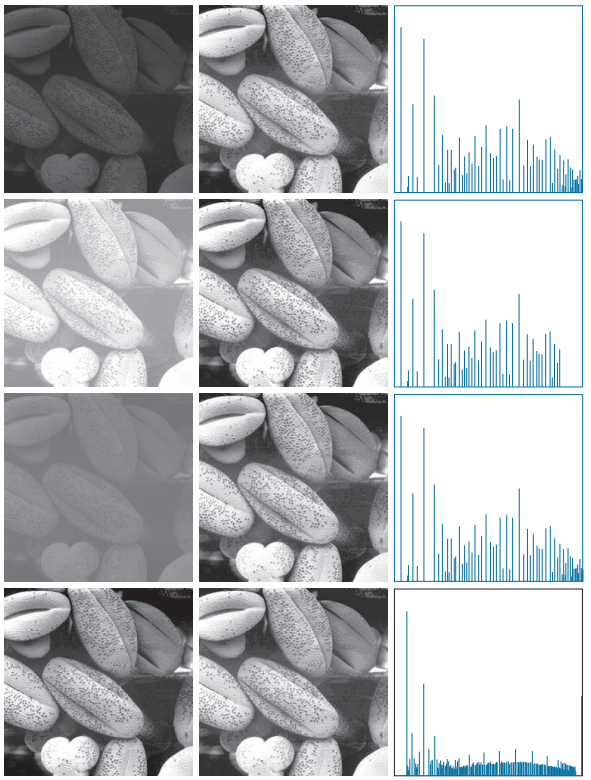
\includegraphics[width=0.5\textwidth]{3-3-20.png}
    \caption{Kolom kiri: Citra dari Gambar 3.16. Kolom tengah: Citra hasil ekualisasi histogram yang bersesuaian. Kolom kanan: Histogram dari citra pada kolom tengah (bandingkan dengan histogram pada Gambar 3.16).}
    \label{fig:gambar3.20}
\end{figure}

\begin{figure}[h]
    \centering
    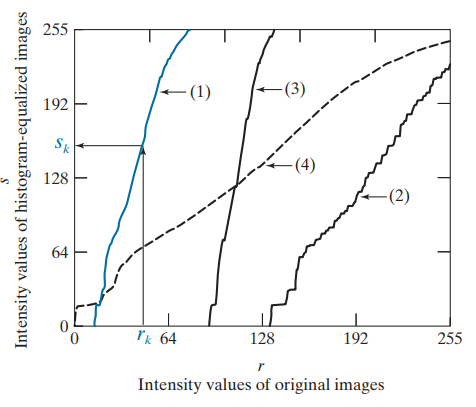
\includegraphics[width=0.5\textwidth]{3-3-21.png}
    \caption{Fungsi transformasi untuk ekualisasi histogram. Transformasi (1) hingga (4) diperoleh menggunakan Persamaan (3-15) dan histogram dari citra pada kolom kiri Gambar 3.20. Pemetaan satu nilai intensitas $r_k$ pada citra 1 ke nilai yang bersesuaian $s_k$ ditunjukkan.}
    \label{fig:gambar3.21}
\end{figure}

\begin{notebox}
\textbf{Hasil:} Citra yang tadinya ``buram'' karena kontras rendah akan menjadi lebih tajam secara otomatis. Lihat \textbf{[FIGURE 3.21]}.
\end{notebox}


\setcounter{figure}{22} % supaya berikutnya jadi 3.21

\begin{figure}[h]
    \centering
    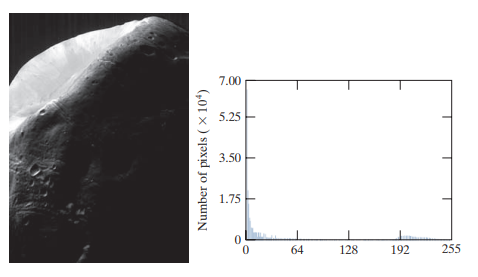
\includegraphics[width=0.5\textwidth]{3-3-23.png}
    \caption{(a) Sebuah citra, dan (b) histogramnya..}
    \label{fig:gambar3.23}
\end{figure}

\begin{figure}[h]
    \centering
    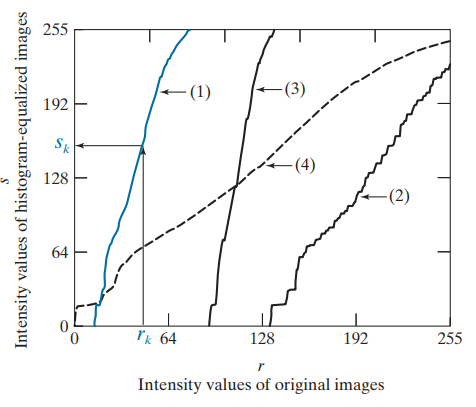
\includegraphics[width=0.5\textwidth]{3-3-21.png}
    \caption{(a) Transformasi ekualisasi histogram yang diperoleh menggunakan histogram pada Gambar 3.23(b).
(b) Citra hasil ekualisasi histogram.
(c) Histogram dari citra yang telah diekualisasi.}
    \label{fig:gambar3.24}
\end{figure}

\begin{notebox}
\textbf{Pertanyaan Reflektif:} Jika HE bisa memperbaiki kontras secara otomatis, mengapa kita masih membutuhkan \textit{Histogram Matching (Spesifikasi)}? Petunjuk: terkadang HE membuat citra terlihat ``terlalu terang'' atau tidak natural. Lihat \textbf{[FIGURE 3.24]}.
\end{notebox}

\subsection{Histogram Matching (Spesifikasi Histogram)}

Histogram Matching memungkinkan kita menentukan \textit{bentuk histogram target} yang diinginkan, bukan hanya seragam. Ini berguna ketika kita ingin mencocokkan penampilan dua citra berbeda (misalnya dalam mosaik satelit).

Langkah-langkahnya:
\begin{enumerate}
  \item Hitung CDF dari citra asal: $s = T(r)$.
  \item Hitung CDF dari distribusi target: $G(z)$.
  \item Cari pemetaan $z = G^{-1}(s)$.
\end{enumerate}

\subsection{Contoh Kode: Histogram Equalization}

\begin{lstlisting}[language=Python, caption={Histogram Equalization dari nol (tanpa OpenCV)}]
import numpy as np
from PIL import Image
import matplotlib.pyplot as plt

def histogram_equalization(img_gray):
    """
    img_gray: numpy array 2D, nilai [0, 255]
    """
    L = 256
    M, N = img_gray.shape
    total_pixels = M * N

    # 1. Hitung histogram
    hist = np.zeros(L, dtype=np.float64)
    for val in img_gray.flatten():
        hist[val] += 1

    # 2. Normalisasi -> PDF
    pdf = hist / total_pixels

    # 3. Hitung CDF
    cdf = np.cumsum(pdf)

    # 4. Buat lookup table (LUT) transformasi
    lut = np.floor((L - 1) * cdf).astype(np.uint8)

    # 5. Terapkan ke citra
    img_eq = lut[img_gray]
    return img_eq, hist, lut

img = np.array(Image.open("image.jpg").convert("L"))
img_eq, hist, lut = histogram_equalization(img)

fig, axes = plt.subplots(2, 2, figsize=(10, 8))
axes[0, 0].imshow(img, cmap='gray'); axes[0, 0].set_title('Citra Asli')
axes[0, 1].imshow(img_eq, cmap='gray'); axes[0, 1].set_title('Setelah HE')
axes[1, 0].bar(range(256), hist, width=1); axes[1, 0].set_title('Histogram Asli')
axes[1, 1].hist(img_eq.flatten(), bins=256); axes[1, 1].set_title('Histogram Setelah HE')
plt.tight_layout()
plt.show()
\end{lstlisting}

\begin{tipbox}
\textbf{Tips Praktis:} Dengan \texttt{OpenCV}, HE bisa dilakukan hanya dengan satu baris: \texttt{cv2.equalizeHist(img)}. Implementasi manual di atas berguna untuk memahami mekanismenya secara mendalam.
\end{tipbox}

% ==============================================================================
\section{Dasar Penyaringan Spasial (Bagian 3.4)}
% ==============================================================================

\subsection{Mekanisme: Neighborhood Processing}

Berbeda dengan \textit{point processing}, penyaringan spasial menggunakan \textbf{Neighborhood Processing}. Sebuah jendela kecil bernama \textbf{kernel} (juga disebut \textit{mask}, \textit{filter}, atau \textit{template}) digeser di atas citra piksel demi piksel.

Di setiap posisi, hasil perkalian elemen-per-elemen antara kernel dan area citra di bawahnya dijumlahkan untuk menghasilkan nilai piksel baru.

\subsection{Korelasi vs.\ Konvolusi}

Dua operasi ini sering tertukar. Perbedaan teknisnya penting:

\begin{center}
\begin{tabular}{lll}
\toprule
\textbf{Operasi} & \textbf{Definisi} & \textbf{Penggunaan} \\
\midrule
Korelasi & Kalikan kernel langsung dengan area citra & Filter praktis, CNN \\
Konvolusi & Kernel diputar $180^\circ$ lalu dikalikan & Teori sistem linear \\
\bottomrule
\end{tabular}
\end{center}

\begin{notebox}
\textbf{Catatan Penting:} Untuk kernel yang \textit{simetris} (seperti Gaussian), korelasi dan konvolusi menghasilkan output yang \textit{identik}. Perbedaan hanya muncul pada kernel asimetris.
\end{notebox}

\textbf{Rumus Konvolusi 2D:}
\begin{equation}
  (w * f)(x, y) = \sum_{s=-a}^{a} \sum_{t=-b}^{b} w(s,t)\, f(x-s,\, y-t)
  \label{eq:convolution_2d}
\end{equation}

\textbf{Rumus Korelasi 2D:}
\begin{equation}
  (w \star f)(x, y) = \sum_{s=-a}^{a} \sum_{t=-b}^{b} w(s,t)\, f(x+s,\, y+t)
  \label{eq:correlation_2d}
\end{equation}

\subsection{Padding: Menangani Tepi Citra}

Saat kernel diaplikasikan di tepi citra, sebagian area kernel berada di luar batas citra. Beberapa strategi penanganan:

\begin{itemize}
  \item \textbf{Zero Padding}: isi area luar dengan nol. Paling sederhana, bisa membuat tepi gelap.
  \item \textbf{Reflect Padding}: cerminkan nilai piksel. Lebih natural untuk banyak kasus.
  \item \textbf{Replicate Padding}: ulangi piksel tepi. Umum digunakan.
\end{itemize}

\subsection{Contoh Kode: Konvolusi 2D Manual}

\begin{lstlisting}[language=Python, caption={Implementasi konvolusi 2D dari nol}]
import numpy as np

def convolve2d(image, kernel):
    """
    Konvolusi 2D dengan zero-padding.
    image : numpy array 2D
    kernel: numpy array 2D (ukuran ganjil x ganjil)
    """
    # Rotasi kernel 180 derajat untuk konvolusi
    kernel_rot = np.rot90(kernel, 2)

    kh, kw = kernel_rot.shape
    pad_h, pad_w = kh // 2, kw // 2

    # Zero padding
    padded = np.pad(image, ((pad_h, pad_h), (pad_w, pad_w)), mode='constant')

    H, W = image.shape
    output = np.zeros_like(image, dtype=np.float64)

    for i in range(H):
        for j in range(W):
            region = padded[i:i+kh, j:j+kw]
            output[i, j] = np.sum(region * kernel_rot)

    return output

# Contoh penggunaan dengan kernel sederhana (identitas)
identity_kernel = np.array([[0, 0, 0],
                             [0, 1, 0],
                             [0, 0, 0]])
img = np.array([[100, 120, 80],
                [90,  150, 110],
                [70,  130, 95]])
result = convolve2d(img, identity_kernel)
print(result)  # Harus sama dengan img
\end{lstlisting}

% ==============================================================================
\section{Penyaringan Smoothing / Lowpass (Bagian 3.5)}
% ==============================================================================

\subsection{Tujuan}

Filter \textit{smoothing} bertujuan mengurangi noise atau menghilangkan detail kecil yang tidak relevan dengan cara mengaburkan (\textit{blurring}) citra. Dalam perspektif frekuensi, filter ini menekan komponen frekuensi tinggi (detail) sambil mempertahankan komponen frekuensi rendah (struktur besar).

\subsection{Box Filter (Average Filter)}

Mengambil rata-rata sederhana dari semua piksel dalam jendela berukuran $n \times n$.

\begin{equation}
  \mathbf{K}_{\text{box}} = \frac{1}{n^2}
  \begin{bmatrix}
    1 & 1 & \cdots & 1 \\
    1 & 1 & \cdots & 1 \\
    \vdots & & \ddots & \vdots \\
    1 & 1 & \cdots & 1
  \end{bmatrix}
  \label{eq:box_filter}
\end{equation}

\textbf{Kelebihan:} Sederhana dan cepat secara komputasi.

\textbf{Kekurangan:} Menghasilkan efek ``kotak'' (\textit{ringing}) pada tepi karena semua tetangga diberi bobot sama.

\setcounter{figure}{30}

\begin{figure}[htbp]
\centering
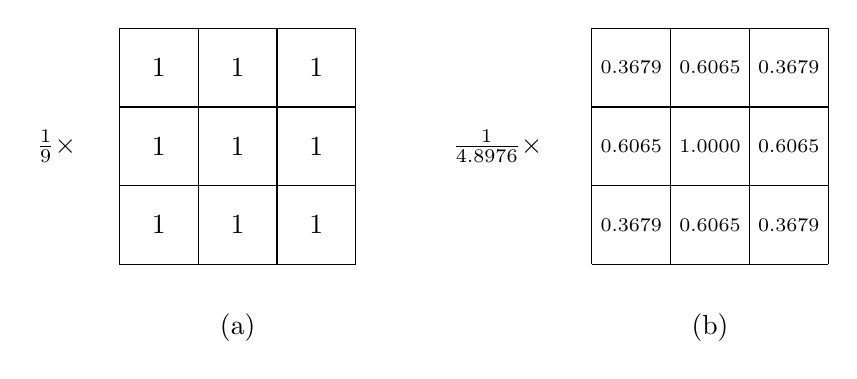
\begin{tikzpicture}

% --- (a) BOX KERNEL ---
\draw (0,0) grid (3,3);

\foreach \x in {0.5,1.5,2.5}
  \foreach \y in {0.5,1.5,2.5}
    \node at (\x,\y) {1};

\node at (1.5,-0.8) {(a)};
\node at (-0.8,1.5) {$\frac{1}{9}\times$};

% --- (b) GAUSSIAN KERNEL ---
\begin{scope}[xshift=6cm]
\draw (0,0) grid (3,3);

\node at (0.5,2.5) {\scriptsize 0.3679};
\node at (1.5,2.5) {\scriptsize 0.6065};
\node at (2.5,2.5) {\scriptsize 0.3679};

\node at (0.5,1.5) {\scriptsize 0.6065};
\node at (1.5,1.5) {\scriptsize 1.0000};
\node at (2.5,1.5) {\scriptsize 0.6065};

\node at (0.5,0.5) {\scriptsize 0.3679};
\node at (1.5,0.5) {\scriptsize 0.6065};
\node at (2.5,0.5) {\scriptsize 0.3679};

\node at (1.5,-0.8) {(b)};
\node at (-1.2,1.5) {$\frac{1}{4.8976}\times$};

\end{scope}

\end{tikzpicture}

\caption{Contoh kernel smoothing: (a) adalah kernel kotak (\textit{box kernel}); (b) adalah kernel Gaussian.}
\label{fig:gambar3.31}

\end{figure}

Lihat hasil box filter pada \textbf{[FIGURE 3.31a]}.

\subsection{Gaussian Filter}

Memberikan bobot lebih besar pada piksel yang lebih dekat ke pusat kernel. Dimodelkan dengan fungsi Gaussian 2D:

\begin{equation}
  G(s,t) = K \cdot e^{-\dfrac{s^2 + t^2}{2\sigma^2}}
  \label{eq:gaussian_function}
\end{equation}

di mana $\sigma$ adalah standar deviasi yang mengontrol ``lebar'' pengaburan, dan $K$ adalah konstanta normalisasi.

\textbf{Kelebihan:}
\begin{itemize}
  \item Hasil lebih halus dan natural.
  \item Bersifat \textit{isotropik} (efek sama ke segala arah).
  \item Dapat dipisahkan menjadi dua filter 1D (efisien secara komputasi).
\end{itemize}

Contoh kernel Gaussian $3\times3$ ($\sigma \approx 1$):
\begin{equation}
  \mathbf{K}_{\text{gauss}} \approx \frac{1}{16}
  \begin{bmatrix}
    1 & 2 & 1 \\
    2 & 4 & 2 \\
    1 & 2 & 1
  \end{bmatrix}
  \label{eq:gaussian_kernel_example}
\end{equation}

Lihat hasil Gaussian filter pada \textbf{[FIGURE 3.31b]}.

\subsection{Median Filter (Non-Linear)}

Berbeda dari dua filter sebelumnya, median filter \textit{bukan} filter linear. Nilai piksel baru adalah \textbf{nilai median} dari semua piksel dalam jendela.

\textbf{Keunggulan utama:} Sangat efektif menghilangkan \textit{salt-and-pepper noise} (piksel yang tiba-tiba bernilai 0 atau 255) tanpa merusak tepi (\textit{edge}) citra -- sesuatu yang tidak bisa dilakukan filter linear dengan baik.

\begin{tipbox}
\textbf{Mengapa Median Filter Bekerja?} Piksel \textit{salt-and-pepper} adalah \textit{outlier} yang nilainya jauh dari tetangga sekitarnya. Operasi rata-rata (mean) dipengaruhi oleh outlier, tapi median tidak -- median selalu memilih nilai ``tengah'' yang lebih representatif.
\end{tipbox}

\subsection{Contoh Kode: Perbandingan Filter Smoothing}

\begin{lstlisting}[language=Python, caption={Membandingkan Box, Gaussian, dan Median Filter}]
import numpy as np
from PIL import Image
import matplotlib.pyplot as plt
from scipy import ndimage

# Load citra dan tambah salt-and-pepper noise
img = np.array(Image.open("image.jpg").convert("L"), dtype=np.float64)
noise_mask = np.random.choice([0, 1, 2], size=img.shape, p=[0.05, 0.05, 0.90])
img_noisy = img.copy()
img_noisy[noise_mask == 0] = 0    # pepper
img_noisy[noise_mask == 1] = 255  # salt

# 1. Box Filter
box_kernel = np.ones((5, 5)) / 25.0
img_box = ndimage.convolve(img_noisy, box_kernel)

# 2. Gaussian Filter
img_gauss = ndimage.gaussian_filter(img_noisy, sigma=1.5)

# 3. Median Filter
img_median = ndimage.median_filter(img_noisy, size=5)

# Visualisasi
fig, axes = plt.subplots(1, 4, figsize=(16, 4))
for ax, title, im in zip(axes,
    ['Noisy', 'Box (5x5)', 'Gaussian (sigma=1.5)', 'Median (5x5)'],
    [img_noisy, img_box, img_gauss, img_median]):
    ax.imshow(np.clip(im, 0, 255).astype(np.uint8), cmap='gray')
    ax.set_title(title); ax.axis('off')
plt.tight_layout(); plt.show()
\end{lstlisting}

% ==============================================================================
\section{Penyaringan Sharpening / Highpass (Bagian 3.6)}
% ==============================================================================

\subsection{Prinsip Dasar: Penajaman sebagai Diferensiasi}

Jika \textit{smoothing} identik dengan integrasi (menghaluskan perubahan), maka \textbf{sharpening} identik dengan \textbf{diferensiasi} (memperkuat perubahan). Tepi pada citra adalah area di mana intensitas berubah tajam -- persis apa yang dideteksi oleh turunan.

\subsection{Laplacian: Turunan Orde Kedua}

Laplacian adalah operator diferensial orde kedua yang paling populer untuk penajaman citra karena bersifat \textit{isotropik}.

\textbf{Definisi kontinu:}
\begin{equation}
  \nabla^2 f = \frac{\partial^2 f}{\partial x^2} + \frac{\partial^2 f}{\partial y^2}
  \label{eq:laplacian_continuous}
\end{equation}

\textbf{Bentuk diskrit} (aproksimasi untuk piksel):
\begin{equation}
  \nabla^2 f(x,y) = f(x+1,y) + f(x-1,y) + f(x,y+1) + f(x,y-1) - 4f(x,y)
  \label{eq:laplacian_discrete}
\end{equation}

\textbf{Kernel Laplacian} yang bersesuaian:
\begin{equation}
  \mathbf{L}_1 =
  \begin{bmatrix}
    0 &  1 & 0 \\
    1 & -4 & 1 \\
    0 &  1 & 0
  \end{bmatrix}
  \qquad \text{atau (dengan diagonal):} \qquad
  \mathbf{L}_2 =
  \begin{bmatrix}
    1 &  1 & 1 \\
    1 & -8 & 1 \\
    1 &  1 & 1
  \end{bmatrix}
  \label{eq:laplacian_kernels}
\end{equation}

\textbf{Cara menggunakannya untuk menajamkan citra:}
\begin{equation}
  g(x,y) = f(x,y) - \nabla^2 f(x,y)
  \label{eq:laplacian_sharpening_op}
\end{equation}

(tanda minus karena Laplacian menghasilkan nilai negatif di puncak tepi)
\setcounter{figure}{43}

\begin{figure}[h]
    \centering
    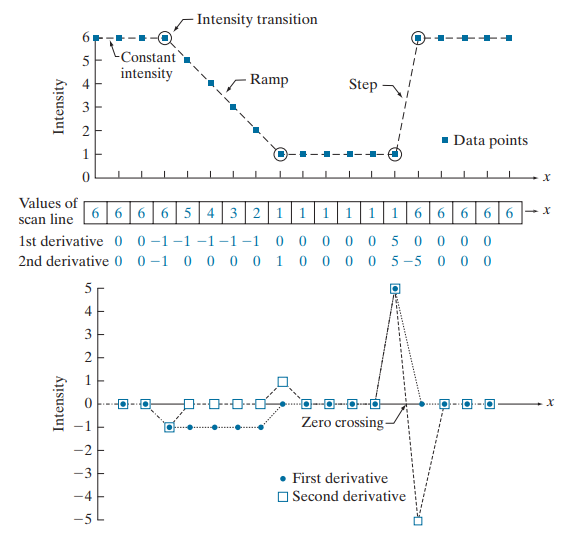
\includegraphics[width=0.5\textwidth]{3-3-44.png}
    \caption{(a) Sebagian dari garis pindai horizontal pada sebuah citra, yang menunjukkan tepi ramp dan step, serta segmen konstan.
(b) Nilai-nilai garis pindai tersebut dan turunannya.
(c) Plot turunan, yang menunjukkan titik potong nol. Pada (a) dan (c), titik-titik dihubungkan dengan garis putus-putus sebagai bantuan visual..}
    \label{fig:gambar3.44}
\end{figure}


\begin{figure}[htbp]
\centering
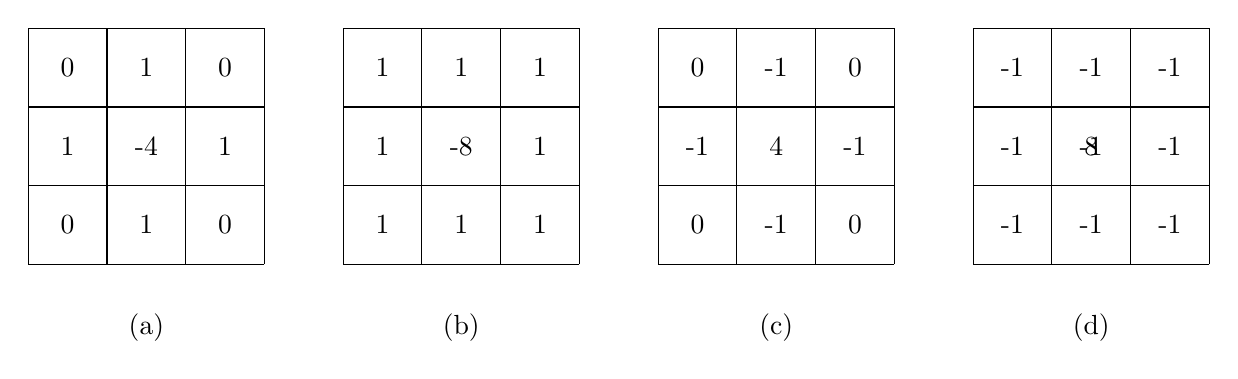
\begin{tikzpicture}

% ukuran kotak
\def\s{1}

% --- (a) ---
\begin{scope}
\draw (0,0) grid (3*\s,3*\s);

\node at (0.5,2.5) {0};
\node at (1.5,2.5) {1};
\node at (2.5,2.5) {0};

\node at (0.5,1.5) {1};
\node at (1.5,1.5) {-4};
\node at (2.5,1.5) {1};

\node at (0.5,0.5) {0};
\node at (1.5,0.5) {1};
\node at (2.5,0.5) {0};

\node at (1.5,-0.8) {(a)};
\end{scope}

% --- (b) ---
\begin{scope}[xshift=4cm]
\draw (0,0) grid (3*\s,3*\s);

\foreach \x in {0.5,1.5,2.5}
  \foreach \y in {0.5,2.5}
    \node at (\x,\y) {1};

\node at (0.5,1.5) {1};
\node at (1.5,1.5) {-8};
\node at (2.5,1.5) {1};

\node at (1.5,-0.8) {(b)};
\end{scope}

% --- (c) ---
\begin{scope}[xshift=8cm]
\draw (0,0) grid (3*\s,3*\s);

\node at (0.5,2.5) {0};
\node at (1.5,2.5) {-1};
\node at (2.5,2.5) {0};

\node at (0.5,1.5) {-1};
\node at (1.5,1.5) {4};
\node at (2.5,1.5) {-1};

\node at (0.5,0.5) {0};
\node at (1.5,0.5) {-1};
\node at (2.5,0.5) {0};

\node at (1.5,-0.8) {(c)};
\end{scope}

% --- (d) ---
\begin{scope}[xshift=12cm]
\draw (0,0) grid (3*\s,3*\s);

\foreach \x in {0.5,1.5,2.5}
  \foreach \y in {0.5,1.5,2.5}
    \node at (\x,\y) {-1};

\node at (1.5,1.5) {8};

\node at (1.5,-0.8) {(d)};
\end{scope}

\end{tikzpicture}

\caption{(a) Kernel Laplacian yang digunakan untuk mengimplementasikan Persamaan (3-53). (b) Kernel yang digunakan untuk mengimplementasikan perluasan dari persamaan tersebut yang mencakup elemen diagonal. (c) dan (d) Dua kernel Laplacian lainnya.}
\label{fig:gambar3.45}

\end{figure}


\begin{figure}[h]
    \centering
    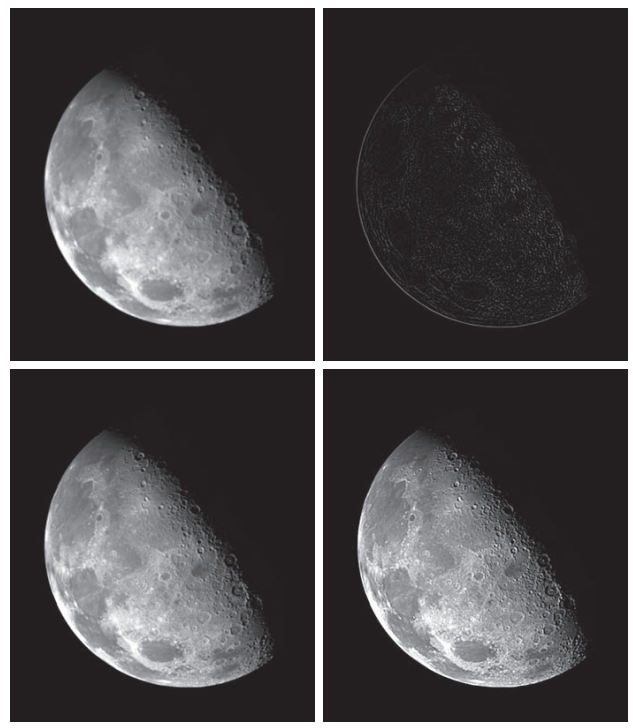
\includegraphics[width=0.5\textwidth]{3-3-46.png}
    \caption{(a) Citra buram dari Kutub Utara bulan. (b) Citra Laplasian yang diperoleh menggunakan kernel pada Gambar 3.45(a). (c) Citra yang dipertajam menggunakan Persamaan (3-54) dengan c=-1c = -1c=-1. (d) Citra yang dipertajam menggunakan prosedur yang sama, tetapi dengan kernel pada Gambar 3.45(b). (Citra asli merupakan milik NASA.)}
    \label{fig:gambar3.46}
\end{figure}

\begin{notebox}
Lihat perbandingan sebelum dan sesudah penajaman dengan Laplacian pada \textbf{[FIGURE 3.46]}.
\end{notebox}

\subsection{Gradient: Turunan Orde Pertama}

Untuk mendeteksi \textit{arah} tepi, digunakan gradient. Operator populer:

\textbf{Sobel Operator:}
\begin{equation}
  \mathbf{G}_x =
  \begin{bmatrix}
    -1 & 0 & 1 \\
    -2 & 0 & 2 \\
    -1 & 0 & 1
  \end{bmatrix}
  \qquad
  \mathbf{G}_y =
  \begin{bmatrix}
    -1 & -2 & -1 \\
     0 &  0 &  0 \\
     1 &  2 &  1
  \end{bmatrix}
  \label{eq:sobel_operator}
\end{equation}

Magnitudo gradient: 
\begin{equation}
  M = \sqrt{G_x^2 + G_y^2}
  \label{eq:gradient_magnitude}
\end{equation}



\begin{notebox}
Perbandingan turunan orde pertama vs.\ orde kedua dalam mendeteksi tepi dan detail halus dapat dilihat pada \textbf{[FIGURE 3.44]}.
\end{notebox}

\subsection{Unsharp Masking}

\textit{Unsharp Masking} adalah teknik penajaman klasik yang berasal dari dunia fotografi film. Langkah-langkahnya:

\begin{enumerate}
  \item Buat citra blur: $\bar{f}(x,y) = \text{Gaussian}(f(x,y))$
  \item Buat ``masker'': $g_{\text{mask}}(x,y) = f(x,y) - \bar{f}(x,y)$
  \item Tambahkan masker ke citra asli:
  \begin{equation}
    g(x,y) = f(x,y) + k \cdot g_{\text{mask}}(x,y)
    \label{eq:unsharp_masking_boost}
  \end{equation}
  di mana $k$ adalah faktor penguat (\textit{boost factor}).
\end{enumerate}

Ketika $k > 1$, teknik ini disebut \textbf{Highboost Filtering}.

\subsection{Contoh Kode: Sharpening dengan Laplacian dan Unsharp Masking}

\begin{lstlisting}[language=Python, caption={Penajaman citra: Laplacian dan Unsharp Masking}]
import numpy as np
from PIL import Image
import matplotlib.pyplot as plt
from scipy import ndimage

img = np.array(Image.open("image.jpg").convert("L"), dtype=np.float64)

# --- 1. Laplacian Sharpening ---
laplacian_kernel = np.array([[ 0,  1,  0],
                              [ 1, -4,  1],
                              [ 0,  1,  0]])

laplacian = ndimage.convolve(img, laplacian_kernel)

# Kurangi citra asli dengan Laplacian (tanda minus karena definisi negatif)
img_laplacian = img - laplacian
img_laplacian = np.clip(img_laplacian, 0, 255)

# --- 2. Unsharp Masking ---
sigma = 3.0
k = 1.5  # boost factor (k > 1 = highboost filtering)

img_blur = ndimage.gaussian_filter(img, sigma=sigma)
mask = img - img_blur
img_unsharp = img + k * mask
img_unsharp = np.clip(img_unsharp, 0, 255)

# Visualisasi
fig, axes = plt.subplots(1, 4, figsize=(16, 4))
data = [
    ('Original', img),
    ('Laplacian Response', laplacian + 128),  # shift untuk visualisasi
    ('Laplacian Sharpened', img_laplacian),
    (f'Unsharp Mask (k={k})', img_unsharp),
]
for ax, (title, im) in zip(axes, data):
    ax.imshow(np.clip(im, 0, 255).astype(np.uint8), cmap='gray')
    ax.set_title(title); ax.axis('off')
plt.tight_layout(); plt.show()
\end{lstlisting}

% ==============================================================================
\section{Ringkasan Perbandingan Filter}
% ==============================================================================

\begin{center}
\renewcommand{\arraystretch}{1.4}
\begin{tabular}{lllll}
\toprule
\textbf{Filter} & \textbf{Tipe} & \textbf{Tujuan} & \textbf{Noise} & \textbf{Tepi} \\
\midrule
Box          & Linear     & Blur/Smoothing     & Kurang efektif  & Rusak \\
Gaussian     & Linear     & Blur/Smoothing     & Efektif         & Agak rusak \\
Median       & Non-linear & Denoising          & Sangat efektif  & Terjaga \\
Laplacian    & Linear     & Sharpening         & Memperkuat noise & Diperkuat \\
Unsharp Mask & Linear     & Sharpening         & Memperkuat noise & Diperkuat \\
Sobel        & Linear     & Deteksi tepi       & Sensitif        & Arah tepi \\
\bottomrule
\end{tabular}
\end{center}

% ==============================================================================
\section{Mini-Latihan (Active Learning)}
% ==============================================================================

\begin{enumerate}[leftmargin=*, label=\textbf{Latihan \arabic*.}]

  \item \textbf{Kernel Laplacian pada Area Seragam} \\
  Dalam Python (menggunakan \texttt{numpy}), jika Anda memiliki kernel Laplacian:
\begin{lstlisting}[language=Python]
kernel = np.array([[0,  1, 0],
                   [1, -4, 1],
                   [0,  1, 0]])
\end{lstlisting}
  Apa yang terjadi jika kernel ini diaplikasikan pada area citra yang intensitasnya seragam (misalnya semua piksel bernilai 100)? Mengapa hasilnya nol?

  \begin{tipbox}
  \textbf{Petunjuk:} Hitung secara manual: $0 + 100 + 0 + 100 + (-4 \times 100) + 100 + 0 + 100 + 0 = ?$ \\
  Apa yang dapat Anda simpulkan tentang sifat Laplacian terhadap wilayah datar?
  \end{tipbox}

  \item \textbf{Orde Pertama vs.\ Orde Kedua} \\
  Berdasarkan \textbf{[FIGURE 3.44]}, jelaskan mengapa turunan orde kedua (Laplacian) lebih baik dalam mendeteksi detail halus dibandingkan turunan orde pertama (Gradient/Sobel).

  \begin{tipbox}
  \textbf{Petunjuk:} Perhatikan respons masing-masing turunan terhadap: (a) tepi tajam (\textit{step edge}), (b) garis tipis, dan (c) area transisi gradual. Turunan orde berapa yang menghasilkan respons puncak (\textit{zero crossing})?
  \end{tipbox}

  \item \textbf{Eksperimen Gamma Correction} \\
  Dengan menggunakan kode di Bagian 2.3, coba nilai $\gamma \in \{0.1, 0.4, 1.0, 2.0, 5.0\}$ pada sebuah citra foto wajah. Dokumentasikan perubahan yang terjadi pada: (a) kecerahan keseluruhan, (b) detail pada area bayangan, dan (c) detail pada area terang.

  \item \textbf{Membandingkan HE vs.\ Tanpa HE} \\
  Ambil sebuah citra yang sangat gelap (misalnya foto malam hari). Terapkan Histogram Equalization, kemudian bandingkan hasilnya dengan menerapkan transformasi gamma $\gamma = 0.3$ secara manual. Mana yang lebih natural? Diskusikan kelebihan dan kekurangan masing-masing pendekatan.

\end{enumerate}

\end{document}